
%%%%%%%%%%%%%%%%%%%%%%% file typeinst.tex %%%%%%%%%%%%%%%%%%%%%%%%%
%
% This is the LaTeX source for the instructions to authors using
% the LaTeX document class 'llncs.cls' for contributions to
% the Lecture Notes in Computer Sciences series.
% http://www.springer.com/lncs       Springer Heidelberg 2006/05/04
%
% It may be used as a template for your own input - copy it
% to a new file with a new name and use it as the basis
% for your article.
%
% NB: the document class 'llncs' has its own and detailed documentation, see
% ftp://ftp.springer.de/data/pubftp/pub/tex/latex/llncs/latex2e/llncsdoc.pdf
%
%%%%%%%%%%%%%%%%%%%%%%%%%%%%%%%%%%%%%%%%%%%%%%%%%%%%%%%%%%%%%%%%%%%


\documentclass[runningheads,a4paper]{llncs}

\usepackage{amssymb}
\setcounter{tocdepth}{3}
\usepackage{graphicx}
\usepackage{multirow}
\usepackage{subfigure}
\usepackage{graphics}

\usepackage{rotating}
\usepackage{verbatim}
\usepackage{float}


\usepackage{url}
\urldef{\mailsa}\path|{alfred.hofmann, ursula.barth, ingrid.haas, frank.holzwarth,|
\urldef{\mailsb}\path|anna.kramer, leonie.kunz, christine.reiss, nicole.sator,|
\urldef{\mailsc}\path|erika.siebert-cole, peter.strasser, lncs}@springer.com|    
\newcommand{\keywords}[1]{\par\addvspace\baselineskip
\noindent\keywordname\enspace\ignorespaces#1}

\usepackage{listings}
\usepackage{color}
\definecolor{javared}{rgb}{0.6,0,0} % for strings
\definecolor{javagreen}{rgb}{0.25,0.5,0.35} % comments
\definecolor{javapurple}{rgb}{0.5,0,0.35} % keywords
\definecolor{javadocblue}{rgb}{0.25,0.35,0.75} % javadoc
 
\lstset{language=Java,
basicstyle=\ttfamily,
keywordstyle=\color{javapurple}\bfseries,
stringstyle=\color{javared},
commentstyle=\color{javagreen},
morecomment=[s][\color{javadocblue}]{/**}{*/},
%numbers=left,
numberstyle=\tiny\color{black},
stepnumber=2,
numbersep=10pt,
tabsize=4,
showspaces=false,
showstringspaces=false}




\begin{document}

\mainmatter  % start of an individual contribution

% first the title is needed
\title{Finding the Effectiveness of ADFD and ADFD+}

% a short form should be given in case it is too long for the running head
\titlerunning{Finding the Effectiveness of ADFD and ADFD+}

% the name(s) of the author(s) follow(s) next
%
% NB: Chinese authors should write their first names(s) in front of
% their surnames. This ensures that the names appear correctly in
% the running heads and the author index.
%
\author{Mian Asbat Ahmad%
%\thanks{Please note that the LNCS Editorial assumes that all authors have usedn the western naming convention, with given names preceding surnames. This determines the structure of the names in the running heads and the author index.}%
\and Manuel Oriol}
%
\authorrunning{Finding the Effectiveness of ADFD and ADFD+} %: Authors' Instructions}
% (feature abused for this document to repeat the title also on left hand pages)

% the affiliations are given next; don't give your e-mail address
% unless you accept that it will be published
\institute{University of York, Department of Computer Science,\\
Deramore Lane, YO10 5GH YORK, United Kingdom\\
%\mailsa\\
%\mailsb\\
%\mailsc\\
%\url{http://www.springer.com/lncs}}
}

%
% NB: a more complex sample for affiliations and the mapping to the
% corresponding authors can be found in the file "llncs.dem"
% (search for the string "\mainmatter" where a contribution starts).
% "llncs.dem" accompanies the document class "llncs.cls".
%

\toctitle{Lecture Notes in Computer Science}
\tocauthor{Authors' Instructions}
\maketitle


\begin{abstract}
The achievement of up-to 50\% better results by Adaptive Random Testing (ART) verses Random Testing (RT) ensures that the pass and fail domains in the input domain are useful and need due consideration during selection of test inputs. The Automated Discovery of Failure Domain (ADFD) and its successor Automated Discovery of Failure Domain+ (ADFD+) techniques, automatically find failures and their domains in a specified range and provides their visualisation.
%They can precisely detect the failure-domain of the identified failure in an effective way. Performing exhaustive testing in a limited region around the failure is the key to the success of ADFD and ADFD+ techniques.

We performed an extensive experimental analysis of Java projects contained in Qualitas Corpus for finding the effectiveness of automated techniques (ADFD and ADFD+). The results obtained were analysed and cross-checked using manual testing. The impact of nature, location, size, type and complexity of failure-domains on the testing techniques were studied. The results provide insights into the effectiveness of automated techniques and a number of lessons for testing researchers and practitioners.





%The abstract should summarize the contents of the paper and shouldcontain at least 70 and at most 150 words. It should be written using the \emph{abstract} environment.
%\keywords{We would like to encourage you to list your keywords within the abstract section}
\keywords{software testing, automated random testing, manual testing, ADFD, Daikon}

\end{abstract}




\section{Introduction}
The input-domain of a given SUT can be divided into two sub-domains. The pass-domain comprises of the values for which the software behaves correctly and the failure-domain comprises of the values for which the software behaves incorrectly. Chan et al.~\cite{chan1996proportional} observed that input inducing failures are contiguous and form certain geometrical shapes. They divided these into point, block and strip failure-domains as shown in Figure~\ref{fig:patterns}. Adaptive Random Testing achieved up to 50\% better performance than random testing by taking into consideration the presence of failure-domains while selecting the test input~\cite{Chen2008}.

\smallskip
\begin{figure} [H]
\centering
\subfigure[Point domain]{
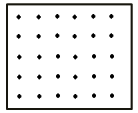
\includegraphics[width=2.5cm,height=2cm]{point.png}
\label{fig:point}
}
\subfigure[Block domain]{
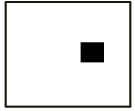
\includegraphics[width=2.5cm,height=2cm]{block.png}
\label{fig:block}
}
\subfigure[Strip domain]{
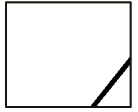
\includegraphics[width=2.5cm,height=2cm]{strip.png}
\label{fig:strip}
}
\smallskip
\caption{Failure domains across input domain~\cite{chan1996proportional}}
\label{fig:patterns}
\end{figure} 

%Adaptive Random Testing (ART) exploited the existence of the failure-domains and resultantly achieved up to 50\% better performance than random testing~\cite{Chen2008}. This was mainly attributed to the better distribution of input which increased the chance of selecting inputs from failure-domains. This insight motivated us to increase our understanding of failure-domains in production software.

The cost of software testing constitute about half of the total cost of software development. Software testing is an expensive but essential process which is particularly time consuming, laborious and error-prone when performed manually. Alternatively, automated software testing may involve higher initial cost but brings the key benefits of lower cost of production, higher productivity, maximum availability, greater reliability, better performance and ultimately proves highly beneficial for any organisation~\cite{Beizer1990}. A case study conducted by Pacheco et al. reveals that the 150 hours of automated testing found more faults in complex .NET code than a test engineer finds in one year by manual testing~\cite{pacheco2008finding}.

We have developed two fully automated techniques ADFD~\cite{ahmad2013adfd} and ADFD+~\cite{ahmad2014adfd2}, which effectively find failures and their domains in a specified range and also provide visualisation of the pass and fail domains. The process is accomplished in two steps. In the first step, an upgraded random testing is used to find the failure. In the second step, exhaustive testing is performed in a limited region around the detected failure in order to identify the domains. The ADFD searches in one-dimension and covers longer range than ADFD+ which is more effective in multi-dimension and covers shorter range.

Three separate tools including YETI, Daikon and JFreeChart have been used in combination to develop ADFD and ADFD+ techniques. The York Extensible Testing Infrastructure~\cite{Oriol2011yeti} is used to test the program automatically with ADFD or ADFD+ strategy. The Daikon~\cite{ernst2007daikon} checks all test executions and automatically generates invariants to present failure-domains quantitatively. The JFreeChart~\cite{gilbert2008jfreechart} facilitates graphical representation of the pass and fail domains.

%Software testing can be performed either automatically or manually. Both the techniques have their own advantages and limitations. The main advantage of automated testing is execution of large number of tests in little time, whereas manual testing utilizes the tester experience to concentrate on error-prone part of the SUT and generate target oriented test cases~\cite{Leitner2007}. 





%The analysis of failures and failure-domains discovered in 57 classes from 25 open source Java projects of Qualitas Corpus through three different techniques---ADFD, ADFD+ and Manual testing---reveals that each is good at uncovering different type of failure-domains and each brings distinct contributions.






The rest of the paper is organized as follows: Section II presents an overview of ADFD+ technique. Section III evaluates and compares ADFD+ technique with Randoop. Section IV reveals results of the experiments. Section V discusses the results. Section VI presents the threats to validity. Section VII presents related work. Finally, Section VIII concludes the study.


 

%%%%%%%%%%%%%%%%%    ADFD and ADFD+   %%%%%%%%%%%%%%%%%%%

%\section{Automated Techniques}
%The two automated techniques used in our experiments are ADFD and ADFD+. A short overview of both the techniques and the enhancements that have been made to the techniques along with a motivating example are given below:
 


%\subsection{Overview of ADFD technique}
%Automated Discovery of Failure Domain is an automated technique for finding and drawing the failure domain of detected failure in the input domain. ADFD searches for failure domain between the specified lower and upper bound in uni-direction. It test and note only the ranges of pass and fail values and uses the scatter graph of the JFreeChart to plot them on the screen. For more details please see \cite{ahmad2013adfd}.

%\subsection{Overview of ADFD+ technique}
%Automated Discovery of Failure Domain+ is an automated technique for finding and drawing the failure domain of detected failure in the input domain. ADFD+ searches for failure domain around the failure in specified range in multi-idirection. It test and note individual value as either pass or fail. The values are drawn using the vector graph of the JFreeChart. For more details please see \cite{ahmad2014adfd2}.


\section{Extension of ADFD and ADFD+ technique}
The ADFD and ADFD+ techniques were extended before performing any experiments, to increase the code coverage, provide information about the identified failure and generate the invariants of the detected failure-domains. This is achieved in the following way.
\begin{enumerate}

\item To increase coverage, the ADFD and ADFD+ techniques were extended to support the testing of methods with byte, short, long, double and float arguments beside the int type arguments.

\item To get details of the failure identified by YETI, the test case generated by YETI is added into the GUI of ADFD and ADFD+ techniques. The test case provides the name of the failing method, the value or values causing the failure and the complete stack trace of the failure. 

\item To auto-generate the invariants of a failure domain, we integrated the tool Daikon in ADFD and ADFD+. Daikon is an automated invariant detector that detect likely invariants in a program~\cite{ernst2007daikon}. The generated invariants are displayed in the GUI of ADFD and ADFD+ after the test is finished. 

\end{enumerate}

\section{Example to explain ADFD and ADFD+ techniques}
To illustrate the difference between the working of ADFD and ADFD+ techniques, we take a simple Java program and test it with the two techniques. It has only one method which receives two integer data types as arguments. It is evident from the program code that an $ArithmeticException$ (divison by zero) failure is generated when the value of variable $x~is~one~of~\{4, 5, 6, 7, 8\}$ and the corresponding value of $y~is~one~of~\{2, 3, 4\}$. The values form a block failure-domain in the input domain. 

\begin{lstlisting}
/** 
* A program with block failure-domain.
* @author (Mian and Manuel)
*/
public class BlockErrorPlotTwoShort {
	public static void blockErrorPlot (int x, int y){
		int z;
		if ((x >= 4) && (x <= 8) && (y == 2))
			{ z = 50/0;}
		if ((x >= 5) && (x <= 8) && (y == 3))
			{ z = 50/0;}
		if ((x >= 6) && (x <= 8) && (y == 4))
			{ z = 50/0;}
	}
}
\end{lstlisting}

The test output generated by ADFD+ technique is presented in Figure~\ref{fig:ADFD+}. The labelled graph correctly shows all the failing values in red whereas the passing values are shown in blue. The invariants are correct indicating that failing values. The test case shows the type of failure, the values causing the first failure and the stack trace of the failure.

The test output generated by ADFD technique is presented in Figure~\ref{fig:ADFD}. The labelled graph shows the correct failing values, however, it scans only in one-dimension therefore both the graph and the invariants failed to identify one of the failing values i.e. when the values of variable $x = 4$. 

Having said this both have their advantages and disadvantage. The ADFD+ uses more resources and not feasible for large range. The ADFD uses very less resources as compared to ADFD and can easily cover long ranges around the failure. It may also be mentioned that both the techniques perform equally well for one-dimensional programs.


\begin{figure}[H]
\centering
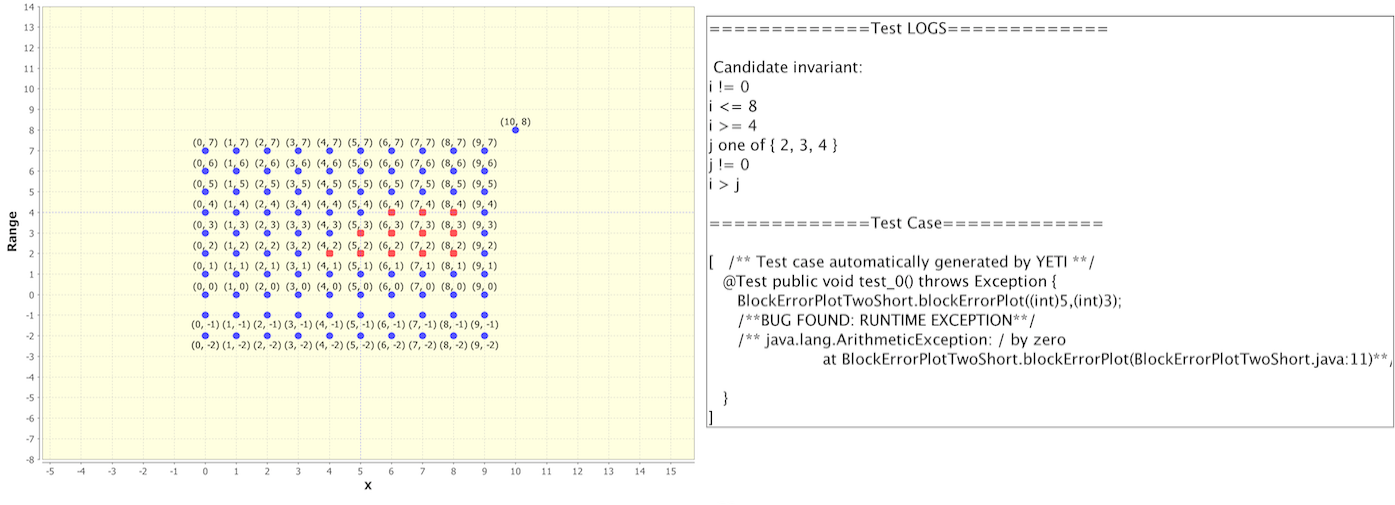
\includegraphics[width= 12.5cm,height=6cm]{adfdPlusCombined.png}
%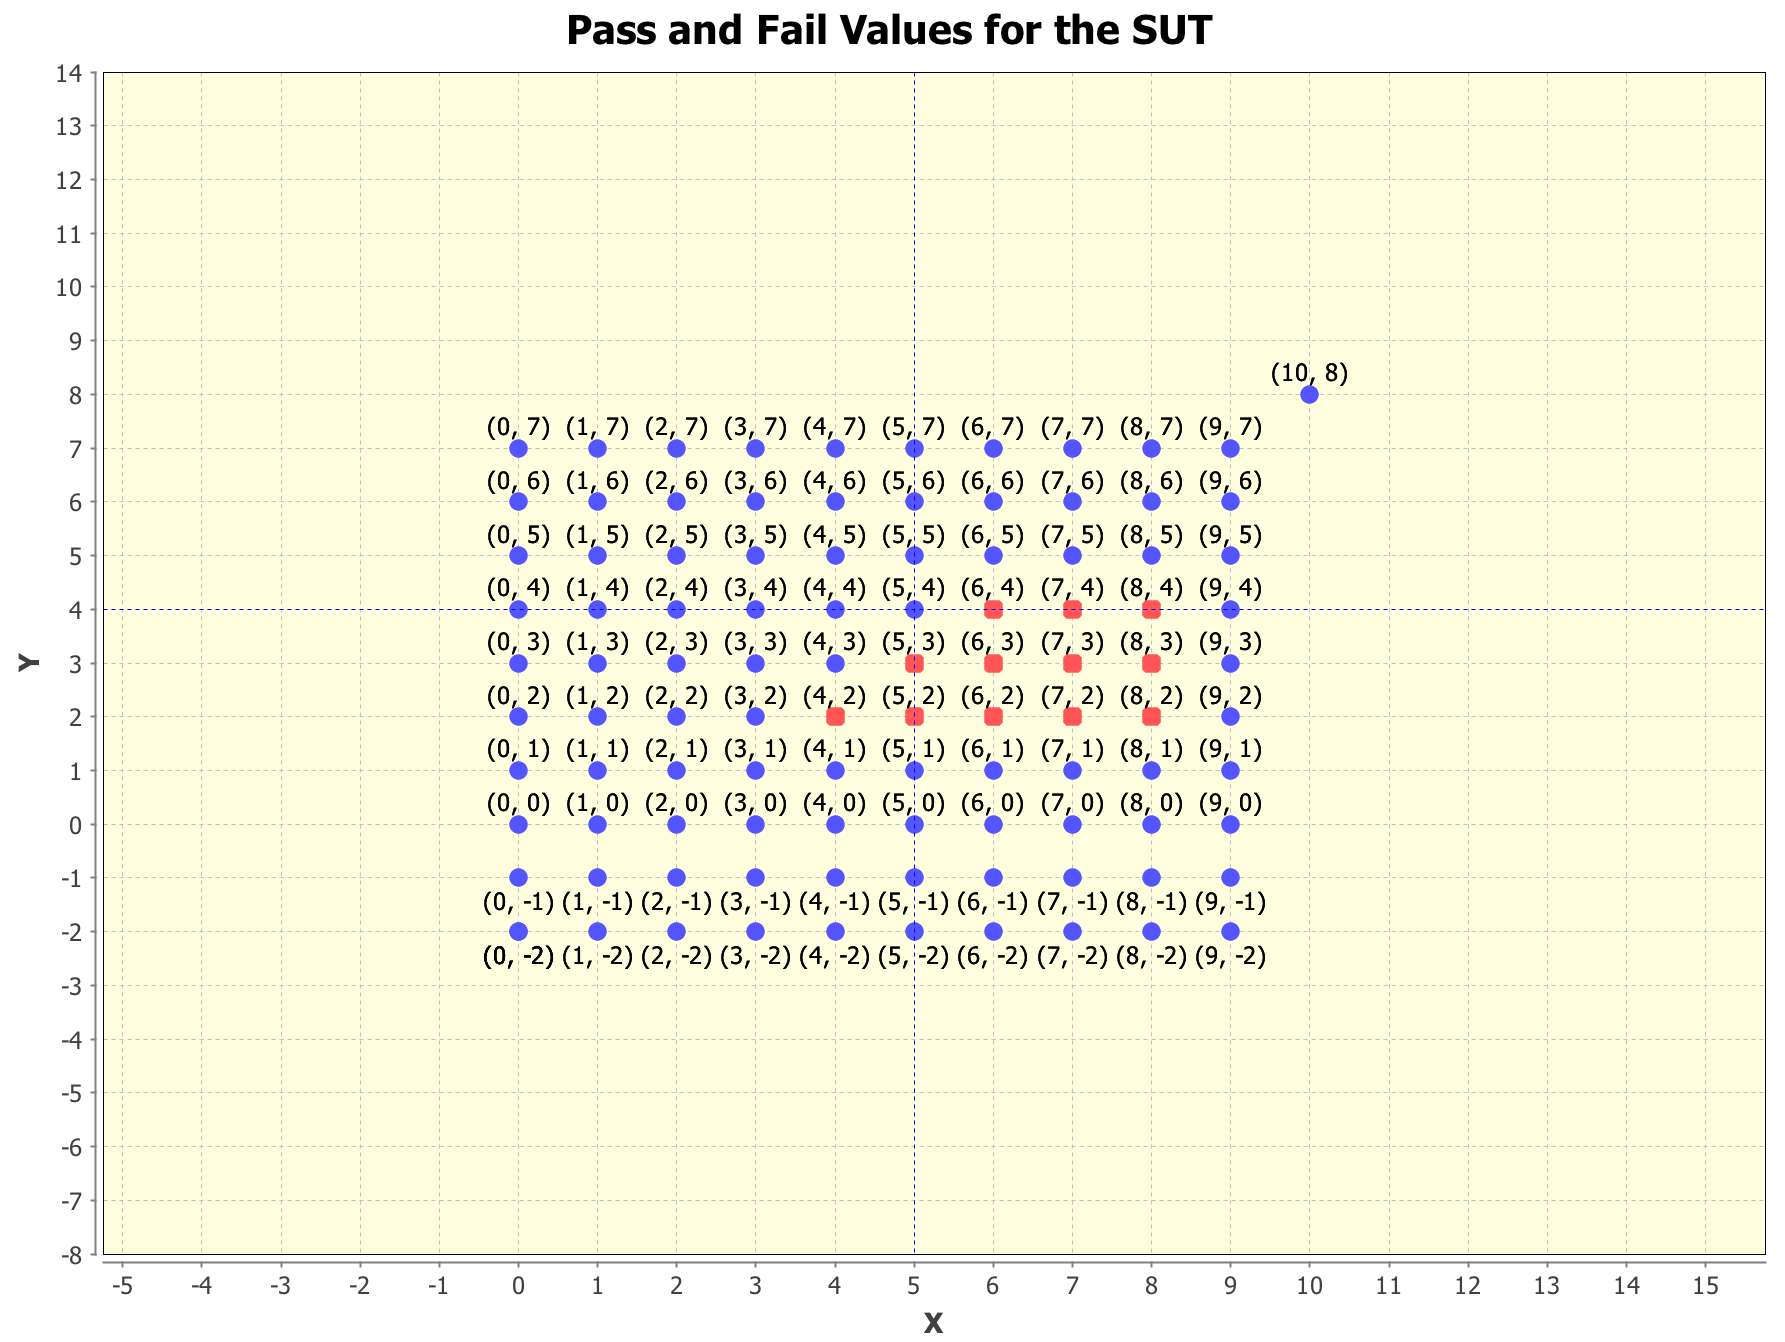
\includegraphics[width= 8.5cm,height=7cm]{adfdPlus1.png}
%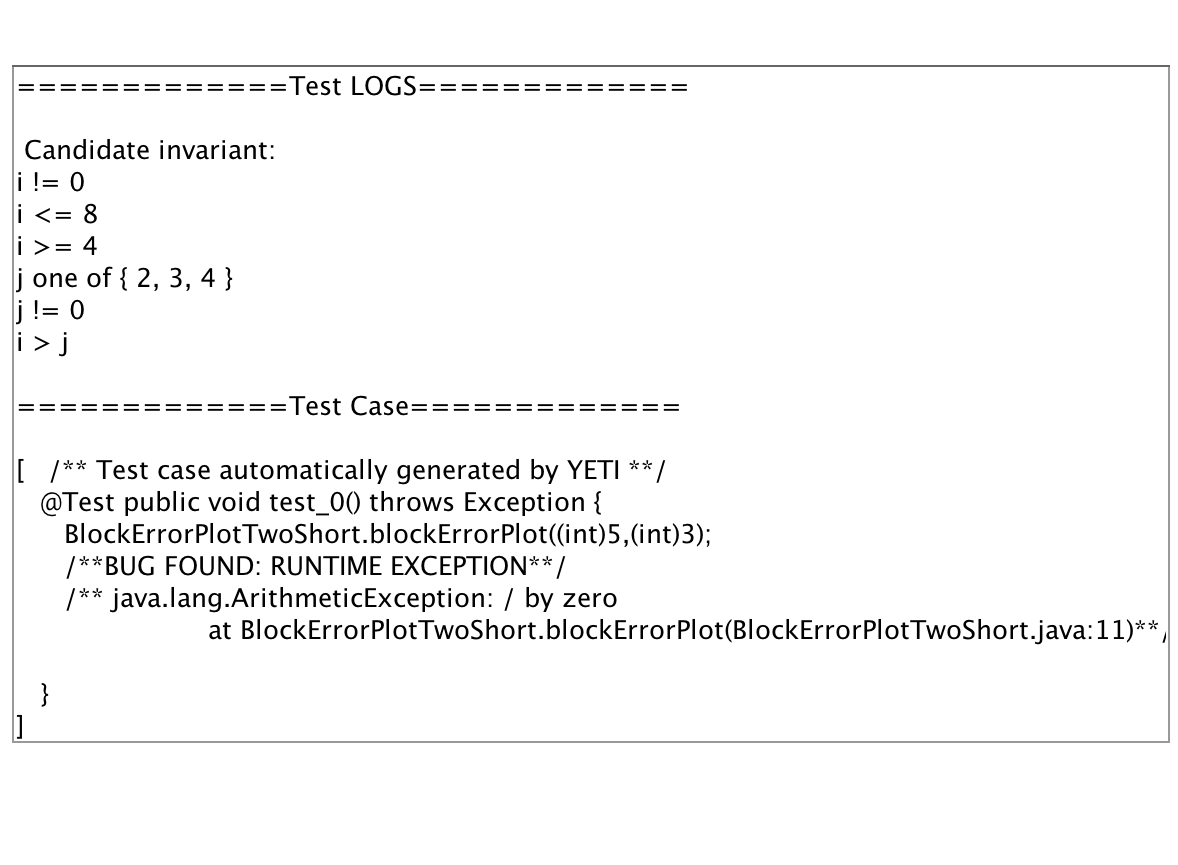
\includegraphics[width= 8.5cm,height=7cm]{adfdPlus2.png}
\caption{Graph, Invariants and Test case generated by ADFD+}
\label{fig:ADFD+}
\end{figure}








\begin{figure}[H]
\centering
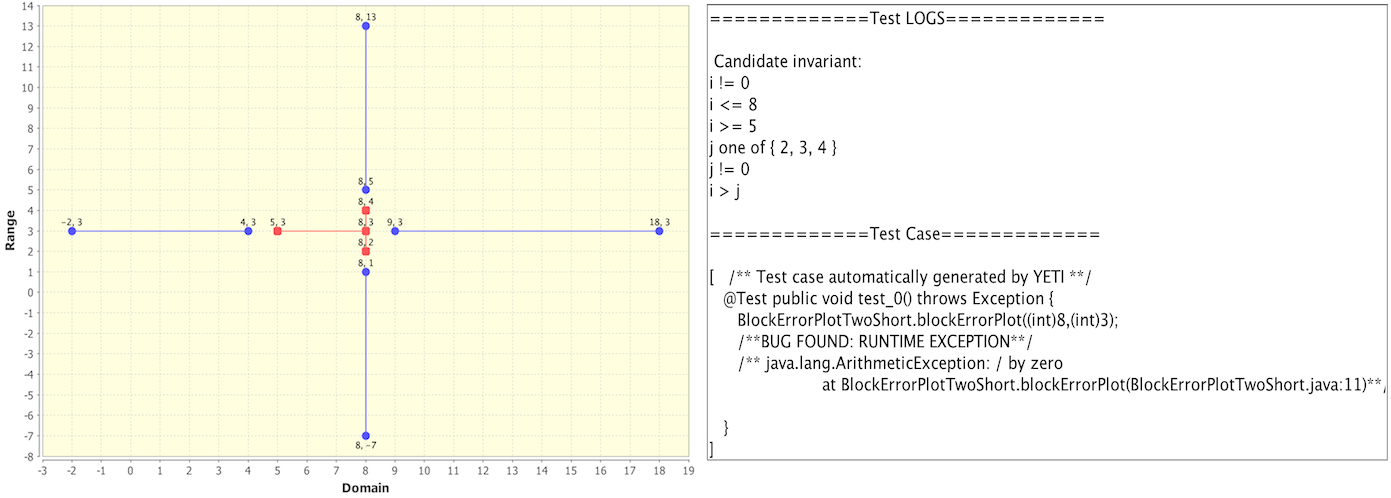
\includegraphics[width= 12.5cm,height=6cm]{adfdCombined.png}
%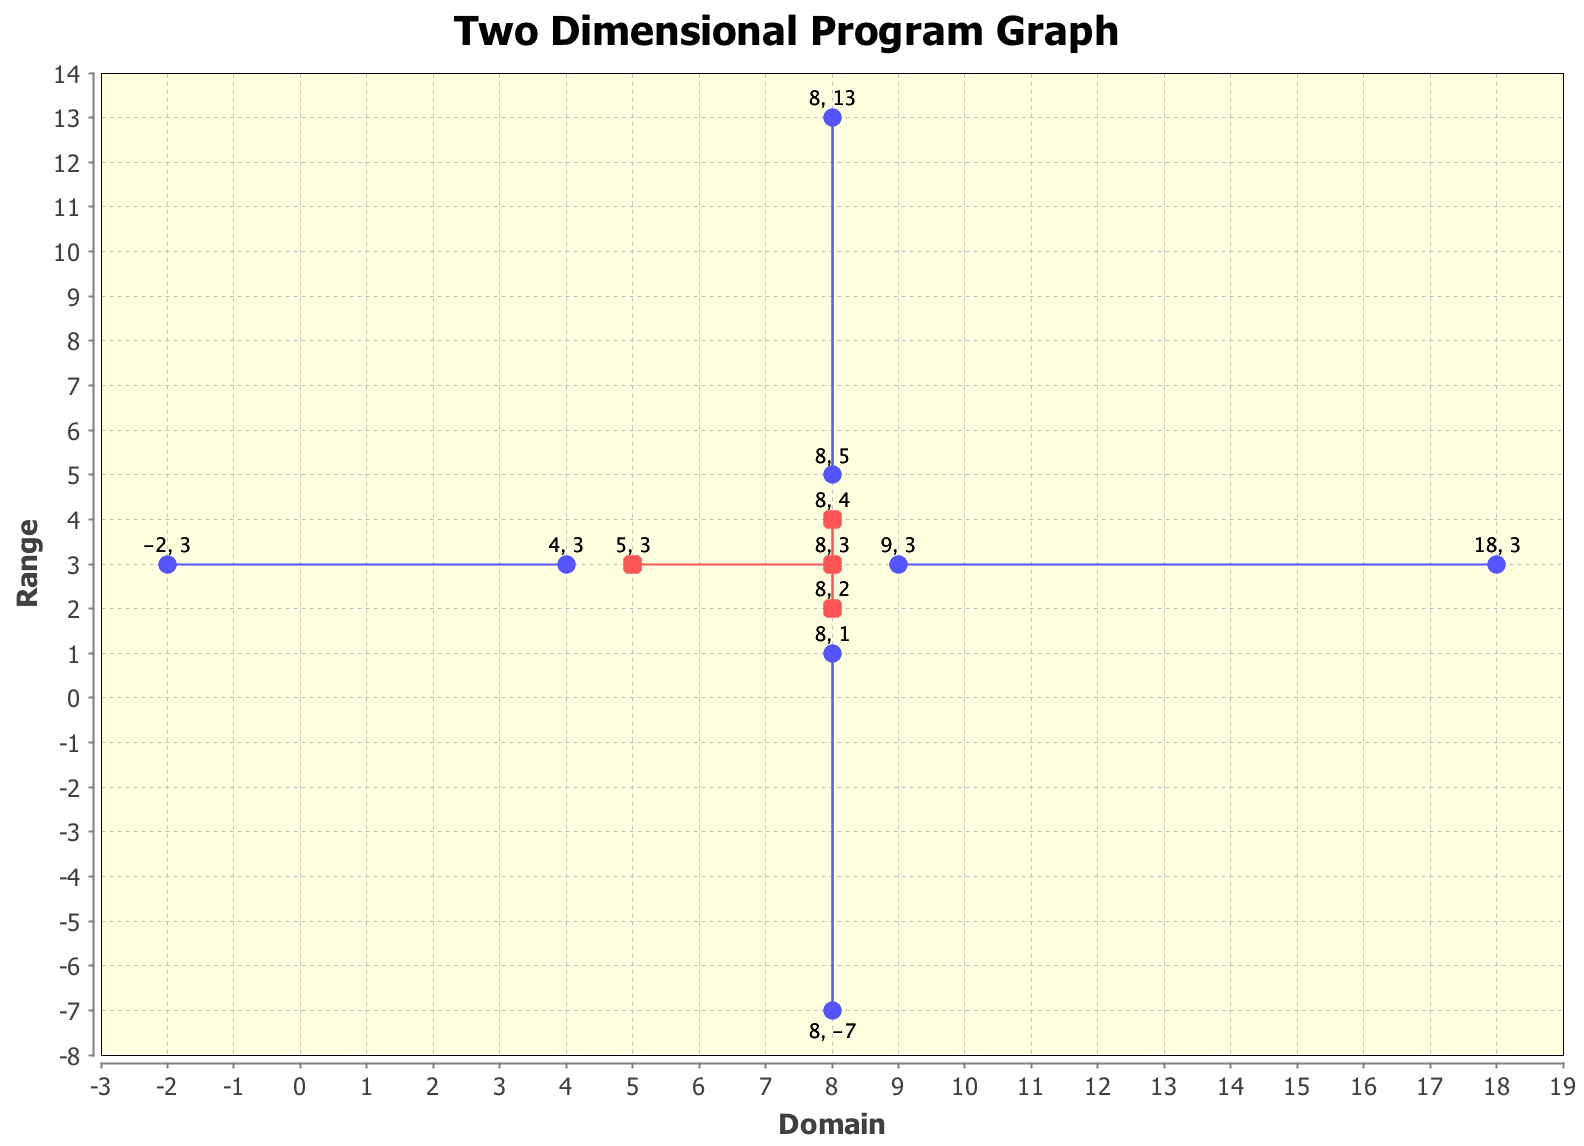
\includegraphics[width= 8.5cm,height=7cm]{adfdAround1.png}
%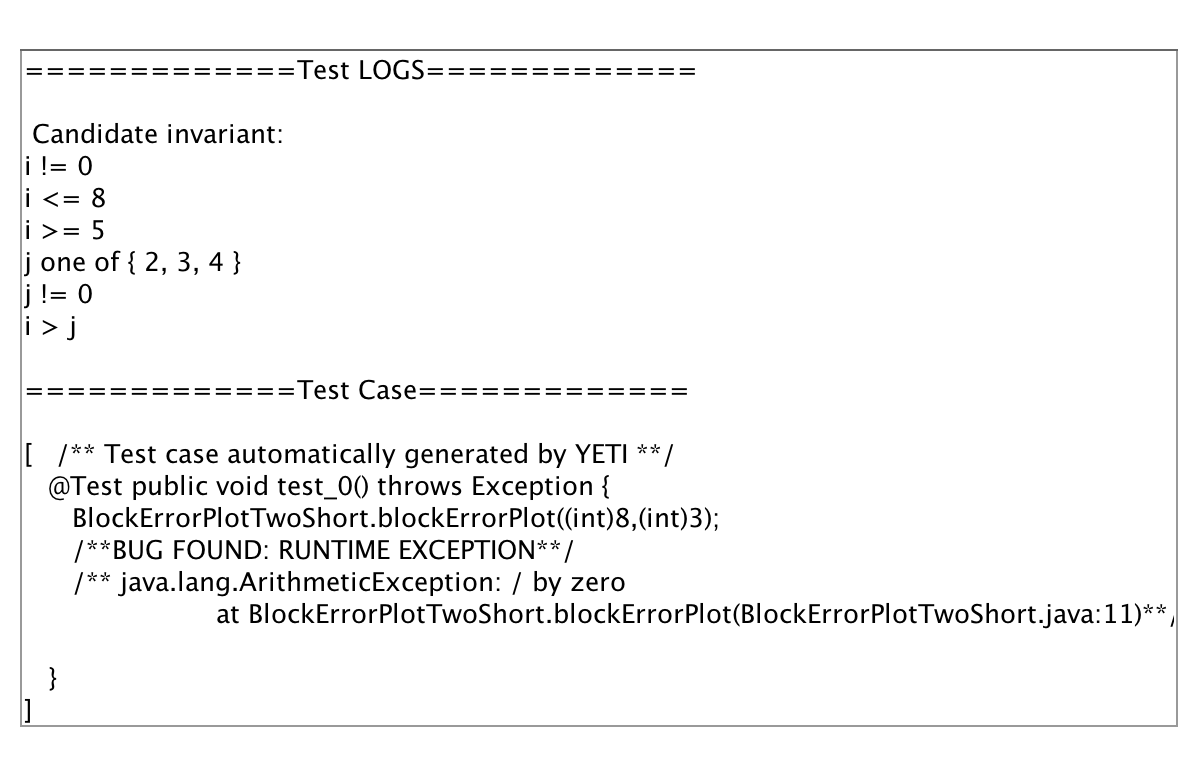
\includegraphics[width= 8.5cm,height=7cm]{adfdAround2.png}
\caption{Graph, Invariants and test case generated by ADFD}
\label{fig:ADFD}
\end{figure}













%\section{Automated Discovery of Failure Domain+}\label{sec:adfd+}
%It is an improved version of ADFD technique developed earlier by Ahmad and Oriol~\cite{ahmad2013adfd}. The technique automatically finds failures, failure domains and present the results in graphical form. In this technique, the test execution is initiated by random+ and continues till the first failure is found in the SUT. The technique then copies the values leading to the failure and the surrounding values to the dynamic list of interesting values. The resultant list provides relevant test data for the remaining test session and the generated test cases are effectively targeted towards finding new failures around the existing failures in the given SUT. \\*
%The improvements made in ADFD+ over ADFD technique are stated as follows.
%\begin{itemize}
%\item ADFD+ generates a single Java file dynamically at run time to plot the failure domains as compared to one Java file per failure in ADFD. This saves sufficient time and makes the execution process quicker.

%\item ADFD+ uses (x, y) vector-series to represent failure domains as opposed to the (x, y) line-series in ADFD. The vector-series allows more flexibility and clarity to represent failure and failure domains.   

%\item ADFD+ takes a single value for the radius within which the strategy searches for a failure domain whereas ADFD takes two values as lower and upper bounds representing x and y-axis respectively. This results in consumption of lower number of test cases for detecting failure domain.

%\item In ADFD+, the algorithm of dynamically generating Java file at run-time has been made simplified and efficient as compared to ADFD resulting in reduced overhead.

%\item In ADFD+, the point, block and strip failure domains generated in the output graph present a clear view of pass and fail domains with individually labelled points of failures as against a less clear view of pass and fail domains and lack of individually labelled points in ADFD. 


%The points are also labelled for clarification. % as shown in Figure~\ref{fig:Workflow}. 

%The difference in representation of fault by ADFD and ADFD+ can be seen in figure .... Figure x is generated by ADFD with lower bound as ... and upper bound as ... While Figure Y is generated by ADFD+ with range ... for the same program given in appendix a. 
%\end{itemize}


%%%%%%%%%%%%%%%%%%%%

%\subsection{Workflow of ADFD+} \label{sec:workflow}
%ADFD+ is a fully automatic technique requiring the user to select radius value and feed the program under test followed by clicking the $Draw Fault Domain$ button for test execution. %The default range value is set to 5 meaning that ADFD+ will search 83 values around the failure. 
%As soon as the button is clicked, YETI comes in to play with ADFD+ strategy to search for failures in the program under test. On finding a failure, the strategy creates a Java file which contains calls to the program on the failing and surrounding values within the specified radius. The Java file is executed after compilation and the results obtained are analysed to separate  pass and fail values which are accordingly stored in the text files. At the end of test, all the values are plotted on the graph with pass values in blue and fail values in red colour as shown in Figure~\ref{fig:adfdPlusExample}.
%\\

%Instead of front end give workflow. It will make more sense. Change the code of the program

%\begin{figure}[ht]
%\centering
%\includegraphics[width= 8.5cm,height=7cm]{adfdPlusWorkflow.png}
%\caption{Workflow of ADFD+}
%\label{fig:Workflow}
%\end{figure}


%%%%%%%%%%%%%%%%%%%%
%ADFD+ is an extension of ADFD's algorithm with more accuracy to find and clarity to plot the failure domain on a graphical chart. Deriving failure domains using ADFD+ is a one click process and all the tester needs to input is the class to test and the range-value for which to search around the found failure. 
%%%%%%%%%%%%%%%%%%%%

%\subsection{Implementation of ADFD+} \label{sec:implementation}
%The ADFD+ technique is implemented in YETI which is available in open-source at \url{http://code.google.com/p/yeti-test/}. A brief overview of YETI is given with the focus on parts relevant to implementation of ADFD+ strategy. \\*
%YETI is a testing tool developed in Java for automatic testing of programs using random strategies. YETI meta-model is language-agnostic which enables it to test 
%programs written in functional, procedural and object-oriented languages. YETI consists of three main parts including core infrastructure for extendibility, strategies section for adjustment of multiple strategies and languages section for supporting multiple languages. Both strategies and languages sections have pluggable architecture for easily incorporating new strategies and languages making YETI a favourable choice for implementing ADFD+ strategy. YETI is also capable of generating test cases to reproduce the failures found during the test session. 
%The strategies section in YETI contains different strategies including random, random+, DSSR and ADFD for selection according to specific needs. ADFD+ strategy is implemented in this section by extending the $YetiADFDStrategy$.

%\begin{figure*}[ht]
%\centering
%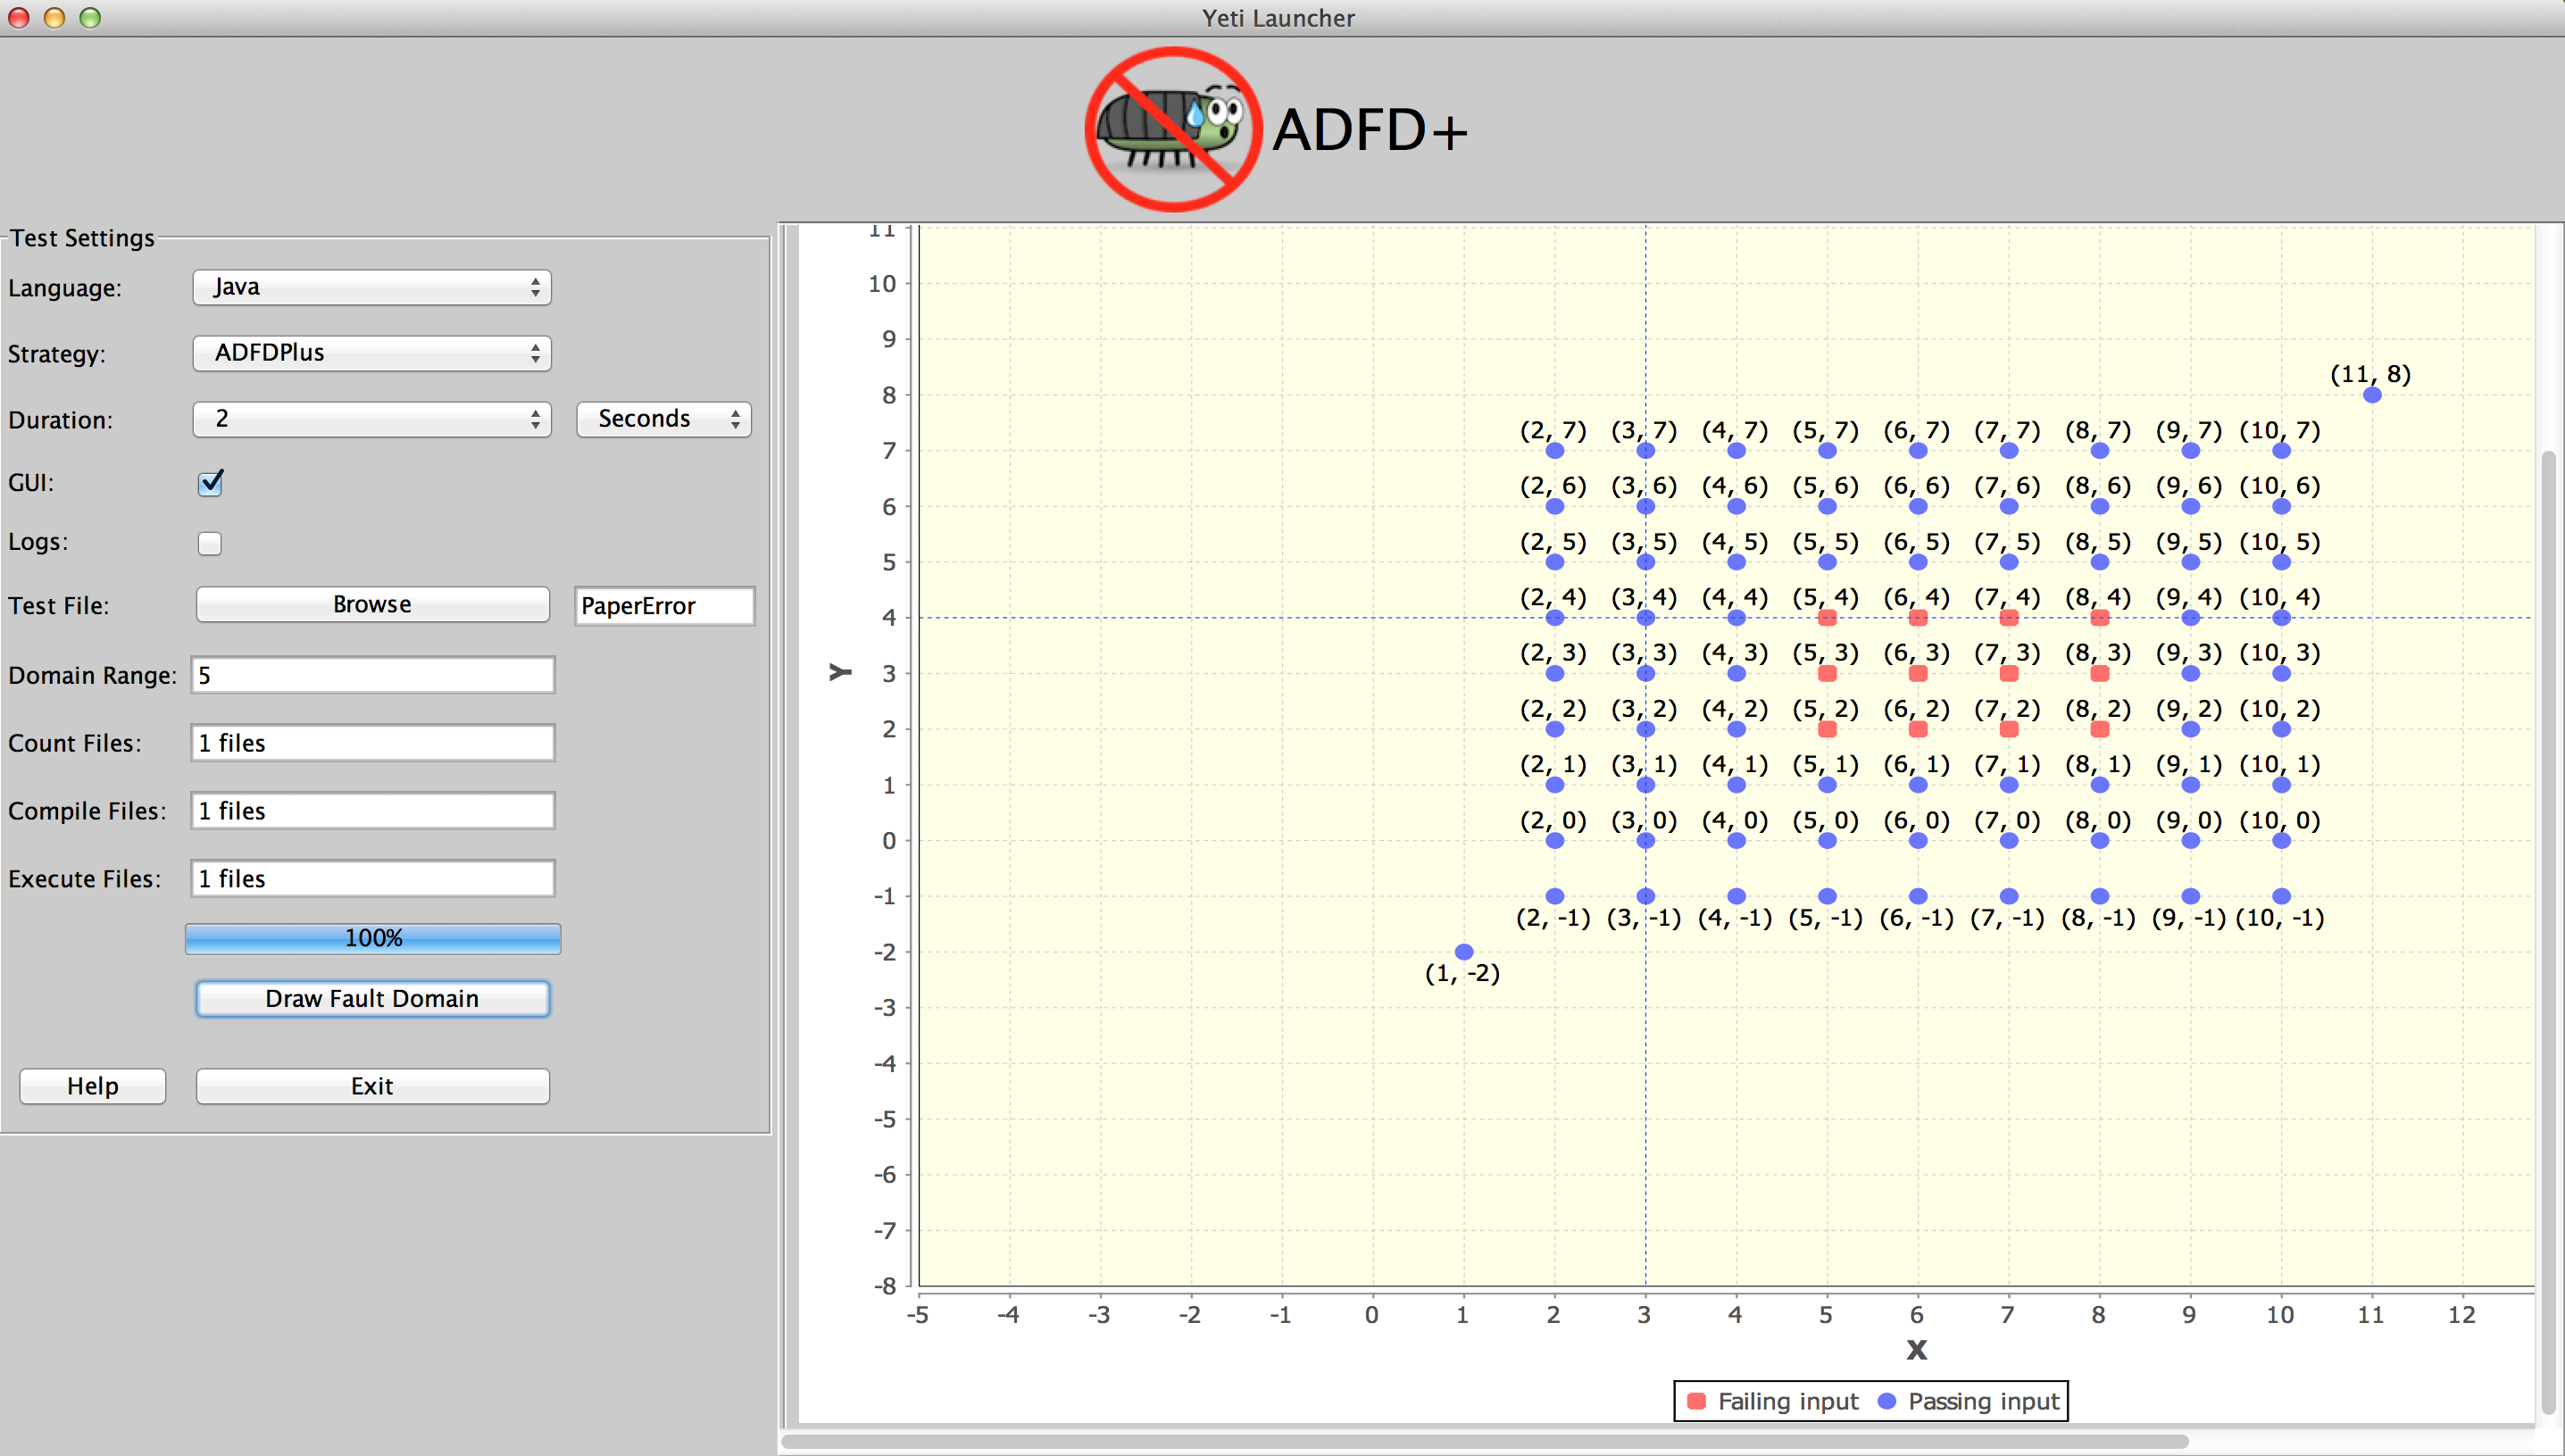
\includegraphics[width=17cm,height=10.3cm]{exampleError.png}
%\caption{The output of ADFD+ for the above code.}
%\label{fig:adfdPlusExample}
%\end{figure*}

%\subsection{Example to illustrate working of ADFD+}
%Suppose we have the following error-seeded class under test. It is evident from the program code that an $ArithmeticException$ (divison by zero) failure is generated when the value of variable $x$ ranges between 5 to 8 and the value of variable $y$ between 2 to 4.

%\begin{lstlisting}
%public class Error {
%  public static void Error (int x, int y){
%    int z;
%    if (((x>=5)&&(x<=8))&&((y>=2)&&(y<=4)))
%		 {
%			 z = 50/0;
%		 }
%   } 
%}
%\end{lstlisting}
%At the beginning of the test, ADFD+ strategy evaluates the given class with the help of YETI and finds the first failure at x = 6 and y = 3. Once a failure is identified ADFD+ uses the surrounding values around it to find a failure domain. The radius of surrounding values is limited to the value set by the user in the $Domain Range$ variable. When the value of $Domain Range$ is set to 5, ADFD+ evaluates a total of 83 values of $x$ and $y$ around the found failure. All evaluated $(x, y)$ values are plotted on a two-dimensional graph with red filled circles indicating fail values and blue filled circles indicating pass values. Figure~\ref{fig:adfdPlusExample} shows that the failure domain forms a block pattern and the boundaries of the failure are $(5, 2), (5, 3),(5, 4), (6, 2), (6, 4), (7, 2), (7, 4), (8, 2), (8, 3), (8, 4)$. 





%%%%%%%%%%%%%%%%%%%%%%%%%%%%%%%%%%%%%%%%%%%%%%%%%
%Randoop maintains two sets called \verb+ErrorSeqs+ and \verb+NonErrorSeqs+ to record the feedback. It extends \verb+ErrorSeqs+ set in case of contract or filter violation and \verb+NonErrorSeqs+ set when no violation is recorded in the feedback. The use of this dynamic feedback evaluation at runtime brings an object to an interesting state. On test completion, \verb+ErrorSeqs+ and \verb+NonErrorSeqs+ are produced as JUnit/NUnit test suite. In terms of coverage and number of faults discovered, Randoop implementing FDRT was compared with JCrasher and JavaPathFinder and 14 libraries of both Java and .Net were evaluated~\cite{visser2004test}. The results showed that Randoop achieved more branch coverage and better fault detection than JCrasher. 

%Daikon is a tool~\cite{ernst2007daikon}, which uses machine-learning technique to automatically generate likely invariants of the program written in C, C++, Java and Pearl. Daikon takes the program and a few test cases as input. The test cases may be either generated manually or by an automated tool. Daikon executes the test cases on the program under test and observes the values that the program computes. At the end of the test session it reports the properties that were true for the observed executions. A feature of Daikon facilitate to process the generated invariants to mitigate non-interesting and redundant invariants. Another feature allows to inserts the generated invariants in to the source code as assertions. The report generated by Daikon is useful in understanding program logic, generating invariants, predicting incompatibilities in component integration, automating theorem proving, repairing inconsistencies in data structures and checking the validity of data streams.

%%%%%%%%%%%%%%%%%    EVALUATION   %%%%%%%%%%%%%%%%%%%%
%\section{Comparison of ADFD+ \& Randoop}\label{sec:eval}
%In order to check the effectiveness and efficiency of ADFD+ we compared it with a random testing tool Randoop. Our subject classes for these experiments were the same that were used in evaluation of ADFD \cite{ahmad2013adfd}. We ran ADFD+ and Randoop for 30 times on each error-seeded one and two dimensional numerical programs, measuring its effectiveness by the total number of test cases used to detect all the failures and its efficiency by the CPU time consumed. 



\section{Evaluation} \label{sec:evaluation}
To evaluate the presence, nature and type of failure-domains in production software we tested the main ``.jar'' files of all the 106 projects in Qualitas Corpus~\cite{}. The source code of the programs containing failure-domains were also evaluated manually to verify the conformance of automated results. Only one and two dimensional numerical programs were selected for evaluation. Every program was tested independently by ADFD, ADFD+ and manual testing. All the programs in which failure-domains were identified are presented in Table~\ref{}.  Due to the absence of contracts and assertions in the code under test, undeclared exceptions were taken as failures in accordance with the previous studies~\cite{ahmad2013adfd, Oriol2012}.


\subsection{Research questions} \label{sec:questions}
The following research questions have been addressed in the study:
\begin{enumerate}
%
\item \textit{If ADFD and ADFD+ techniques capable of correctly identifying and presenting the failure-domains in production software?} %The experimental results claiming the correct identification of ADFD and ADFD+ were based on the purpose build error-seeded programs~\cite{}. To answer the question, we applied the two techniques to all the projects of Qualitas Corpus and examined the results.

%\item \textit{If the graph and invariants generated, correctly represent the failure domains?} %Invariants generated by Daikon can identify the start and stop of the failure domain. To answer this question we compared the generated invariants with the source code and the failure-domain presented in graphical form.
%
%
\item \textit{What are the types and frequency of identified failure-domains?} %There are strategies~\cite{}.  that exploit the presence of block and strip failure-domain to get better results. Therefore identifying the presence of underlying failure-domains in production software can help in high quality of software testing.  To answer the questions, we reviewed all the classes containing failure-domains manually, automatically and graphically.
%
\item \textit{If the nature of identified failure-domains is simple or complex and does it make any difference in its identification by manual and automated techniques?}% An interesting point is to know what failure is responsible for a failure-domain and how difficult it is to identify that failure by manual testing. To answer this question, we studied the test logs and test output of the automated testing and the source code of the program manually to identify the cause and complexity of failures of failure-domains. 

%\item \textit{If the presence of a particular failure-domain can make it easy or hard to find using automated and manual techniques?} 
%Failure-domain can reside in the form of point, block or strip shape in the input domain. To answer this question we analysed the source code of all the programs in which failure-domains were detected.
%

%\item \textit{If the graph generated by ADFD correctly represent the pass and fail domains?} Both the ADFD and ADFD+ techniques generate graphs to represent failure-domains for simplicity. To answer the question we compared the generated graphs with the source code and the invariants generated by Daikon.
%
\item \textit{If obtained results consistent with previous theoretical and practical results presented?}  %As per our knowledge, till now no specific study has been conducted to automatically identify the pass and fail domains however it has been claimed by some researchers~\cite{} that there exist more block and strip patterns then the point patterns. 
%

\end{enumerate}



%\subsection{Randoop} \label{sec:randoop}
%Random tester for object oriented programs (Randoop) is a fully automatic tool, capable of testing Java classes and .Net binaries. It takes as input a set of classes, time limit or number of tests and optionally a set of configuration files to assist testing. Randoop checks for assertion violations, access violations and un-expected program termination in a given class. Its output is a suite of JUnit for Java and NUnit for .Net program. Each unit test in a test suite is a sequence of method calls (hereafter referred as sequence). Randoop builds the sequence incrementally by randomly selecting public methods from the class under test. Arguments for these methods are selected from the pre-defined pool in case of primitive types and as sequence of null values in case of reference type. Randoop uses feedback mechanism to filter out duplicate test cases. 

%The code for the programs under test is given in Appendix~\ref{} while the test details are presented in Table~\ref{table:Results}. 
%Every class was evaluated through $10^5$ calls in each test session of ADFD+.
%\footnote{The total number of tests is equal to $60\times 30\times 3 \times 10^5 = 540\times10^6~tests$.} 




\section{Experimental setup}
We tested all the 4500 classes included in the main jar files of each of the 106 open-source packages contained in Qualitas Corpus~\cite{Tempero2010} using ADFD and ADFD+ technique. The Qualitas Corpus is selected for two reasons: (1) It is a database of open-source Java programs that spans across the whole set of Java applications. (2) It is specially built for empirical research which takes into account a large number of developmental models and programming styles. Each test on average took 40 seconds to complete. The YETI ran for 5 seconds while the remaining time is used for finding failure-domains, generating invariants and drawing graph. The machine took approximately 100 hours to process the experiments. Only the failing one and two dimensional methods with arguments (int, long, float, double and short) were taken in to consideration. This is because at the moment ADFD and ADFD+ are not capable of drawing/handling more than two dimensions. All experiments were conducted with a 64-bit Mac OS X Mountain lion version 10.8.5 running on 2.7 GHz Intel Core i7 with 16 GB (1600 MHz DDR3) of RAM. YETI runs on top of the Java\texttrademark  SE Runtime Environment [version 1.7.0\_45]. The ADFD and ADFD+ executable files are available at \url{https://code.google.com/p/yeti-test/downloads/list/}. 



\section{Results}
We found 57 faulty classes spread across 25 different packages. Results of the experiments are given in Table 1, 2, 3 and 4. All those failure-domains were declared as strip failure-domains in which 100 or more contagious failures were discovered. Accordingly, in 48 out of 57 classes strip failure-domain is detected as shown in Table~\ref{table:stripDomains}. The failure-domains in which 10 or more contagious failures were discovered. The failure-domains in which 5 or less contagious failures were discovered are termed as point failure-domains.There are 4 classes which contain point failure-domain as shown in Table~\ref{table:pointDomains}. The 2 classes contain block failure domain as shown in Table~\ref{table:blockDomains}. The 2 classes contain two types of failure-domains i.e. AnnotationValue with both point and block failure-domain and Token with point and Strip failure-domain as shown in Table~\ref{table:mixDomains}.

The source code of all the 57 classes were analysed manually.

%Randoop at \url{https://randoop.googlecode.com/files/randoop.1.3.3.zip}
%The following two commands were used to run the ADFD+ and Randoop respectively. Both tools were executed with default settings, however, Randoop was provided with a seed value as well.% On running command (1) the ADFD+ starts with a GUI front-end given in Figure \ref{fig:adfdPlusExample}. On running command (2) Randoop starts in CLI mode as there is no GUI.
%\begin{lstlisting}[language=bash]
%$ java -jar adfd_yeti.jar -------------(1)

%$ java randoop.main.Main gentests \
%--testclass=OneDimPointFailDomain \
%--testclass=Values --timelimit=100 ----(2)
%\end{lstlisting}



\begin{table*}[h]
\centering
\noindent\makebox[\textwidth]{
{\renewcommand{\arraystretch}{0.5}
\begin{tabular}{|l|l|l|l|l|l|l|l|l|l|}
\hline

S\#  & Class						& Method 					& ADFD+       								& ADFD     								& Manual							\\
\hline
1	&LeadPipeInputStream 		& LeadPipeInputStream(i)		& I \textgreater= 2147483140				& I 										& I \textgreater~698000000			\\ 
	&                                             &                                             & I \textless= 2147483647  					&										&									\\
2	& BitSet				  		& BitSet.of(i,j)				& I \textless= -1, I \textgreater= -18,			& I one of \{-513, -1\}					& I \textless= -1						\\ 
	&                                             &                                             & J \textless= 7, J \textgreater= -12  			& J one of \{-503, 507\}					& J != 0								\\
3	& ToolPallete			  		& ToolPalette(i,j)				& I \textless= -1, I \textgreater= -18			& I one of \{ -515, -1\}					& I \textless= -1, 					\\ 
	&                                             &                                             & 				  							& J one of \{-509, 501\}					& J any value			   				\\
4	& IntMap			  		& idMap(i)					& I \textless= -1, I \textgreater= -18			& I one of \{-1, -512\} 					& I \textless= -1						\\ 
5	& ExpressionFactory	  		& expressionOfType(i)		& I \textless= 13, I \textgreater= -7			& I one of \{-497, 513\}					& I \textgreater= -2147483648 		\\ 
	&                                             & 				  			& 											&										& I \textless= 2147483647			\\
6	& ArrayStack					& ArrayStack(i)				& I \textgreater= 2147483636				& I one of \{2147483142, 2147483647\}	& I \textgreater~698000000 			\\ 
	&                                             &                                             & I \textless= 2147483647 					& 										&  			   						\\
7	& BinaryHeap				& BinaryHeap(i)				& I \textless= -2147483637					& I one of \{-2147483648, -2147483142\}	& I \textless= 0						 \\
	&                                             &                                             & I \textgreater= -2147483648				& 										&  			   						\\
8	& BondedFifoBuffer			& BoundedFifoBuffer(i)		& I \textless= -2147483639 					& I one of \{-505, 0\} 					& I \textless= 0 						\\
	&                                             &                                             & I \textgreater= -2147483648				& 										&  			   						\\
9	& FastArrayList				& FastArrayList(i)				& I \textless= -2147483641 					& I one of \{-2147483644, -2147483139\}	& I \textless= -1						\\ 
	&                                             &                                             & I \textgreater= -2147483648				& 										&  			   						\\	
10	& StaticBucketMap			& StaticBucketMap(i)			& I \textgreater= 2147483635				& I one of \{2147483140, 2147483647\} 	& I \textgreater~698000000			\\ 
	&                                             &                                             & I \textless= 2147483647					& 										&  			   						\\	
11	& PriorityBuffer				& PriorityBuffer(i)				& I \textless= -1, I \textgreater= -14			& I one of \{-2147483647, -2147483142\}	& I \textless= 0						\\ 
12	& GenericPermuting			& permutation(i,j)			& I \textless= 0, I \textgreater= -18			& I one of \{ -498, 0\}					& I \textless= 0, I \textgreater= 2		\\ 
	&                                             &                                             & 											& I one of \{2, 512\}						& J != 0			   					\\
13	& LongArrayList				& LongArrayList(i)			& I \textless= -2147483640					& I one of \{-510, -1\}					& I \textless= -1						\\ 
	&                                             &                                             & I \textgreater= -2147483648				& 										&  			   						\\
14	& OpenIntDoubleHashMap	& OpenIntDoubleHashMap(i)	& I \textless= -1, I \textgreater= -17			& I one of \{-514, -1\}    					& I \textless= -1						\\ 
15	& ByteVector					& ByteVector(i)				& I \textless= -2147483639					& I one of \{-2147483648, -2147483141\}	& I \textless= -1						\\ 	
	&                                             &                                             & I \textgreater= -2147483648				& 										&  			   						\\	
16	& ElementFactory				& newConstantCollection(i)	& I \textgreater= 2147483636				& I one of \{2147483141, 2147483647\}    & I \textgreater~698000000			\\ 
	&                                             &                                             & I \textless= 2147483647					& 										&  			   						\\	
17	& IntIntMap					& IntIntMap(i)				& I \textless= -2147483638					& I one of \{-2147483644, -2147483139\}	& I \textless= -1						\\ 
	&                                             &                                             & I \textgreater= -2147483648				& 										&  			   						\\	
18	& ObjectIntMap				& ObjectIntMap(i)				& I \textgreater= 2147483640				& I one of \{2147483591, 2147483647\}    & I \textgreater~698000000			\\ 
	&                                             &                                             & I \textless= 2147483647					& 										&  			   						\\	
	& IntObjectMap				& IntObjectMap(i)				& I \textless= -1, I \textgreater= -17			& I \textless= -1, I \textgreater= -518		& I \textless= -1						\\ 
19	& ArchiveUtils				& padTo(i,j)					& I \textgreater= 2147483641 				& I one of \{-497, 513\}					& I any value							\\ 
	&                                             &                                             & I \textless= 2147483647					& J one of \{2147483591, 2147483647\}	& J \textgreater~698000000 	   		\\	
20	& BloomFilter32bit 			& BloomFilter32bit(i,j)			& I \textless= -1								& I one of \{-515, -1\}					& I \textless -1 						\\ 
	&                                             &                                             & I \textgreater= -18							& J may be any value						& J \textless -1 			   			\\	
21	& IntKeyLongValueHashMap	& IntKeyLongValueHashMap(i)	& I \textgreater= 2147483635				& I one of \{2147483590, 2147483647\}	& I \textgreater~698000000			\\ 
	&                                             &                                             & I \textless= 2147483647					& I \textgreater= -518					&  			   						\\	
22	& ObjectCacheHashMap		& ObjectCacheHashMap(i)		& I \textless= -2147483641					& I one of \{-512, 0\}						& I \textless= 0						\\ 
	&                                             &                                             & I \textgreater= -2147483648				& 										&  			   						\\	
23	& ObjToIntMap				& ObjToIntMap(i)				& I \textless= -2147483636					& I one of \{-2147483646, -2147483137\}	& I \textless= -1						\\ 
	&                                             &                                             & I \textgreater= -2147483648				& 										&  			   						\\	
24	& PRTokeniser				& isDelimiterWhitespace(i)		& I \textless= -2								& I one of \{-509, -2\}					& I \textless= -2 					\\ 
	&                                             &                                             & I \textgreater= -18							& I one of \{256, 501\} 					& I \textgreater= 256		   			\\	
25	& PdfAction					& PdfAction(i)				& I \textless= -2147483640 					& I one of \{-514, 0\}						& I \textless= 0 						\\ 
	&                                             &                                             & I \textgreater= -2147483648				& I one of \{6, 496\}						& I \textgreater= 6			   		\\	
26	& PdfLiteral					& PdfLiteral(i)				& I \textless= -1, I \textgreater= -14			& I one of \{-511, -1\}					& I \textless= -1						\\ 
27	& PhysicalEnvironment		& PhysicalEnvironment(i)		& I \textless= -1, I \textgreater= -11			& I one of \{-2147483646, -2147483137\}	& I \textless= -1						\\ 
28	& IntegerArray				& IntegerArray(i)				& I \textgreater= 2147483636				& I one of \{2147483587, 2147483647\}	& I \textgreater~698000000			\\ 
	&                                             &                                             & I \textless= 2147483647					& 										&  			   						\\	
29	& AttributeMap				& AttributeMap(i)				& I \textless= -2147483639					& I one of \{-514, 0\}						& I \textless= 0						\\ 
	&                                             &                                             & I \textgreater= -2147483648				& 										&  			   						\\	
30	& ByteList					& ByteList(i)					& I \textless= -1, I \textgreater= -14			& I one of \{-513, -1\}	 				& I \textless= -1						\\ 
31	& WeakIdentityHashMap		& WeakIdentityHashMap(i)		& I \textgreater= 2147483636				& I one of \{2147483140, 2147483647\}	& I \textgreater 698000000			\\ 
	&                                             &                                             & I \textless= 2147483647					& 										&  			   						\\
32	& AmmoType				& getMunitionsFor(i)			& I \textless= -1								& I one of \{-514, -1\}					& I \textless= -1 					\\ 			
	&                                             &                                             & I \textgreater= -17							& I one of \{93, 496\}						& I \textgreater= 93		   			\\
33	& IntList						& IntList(i,j)					& I \textless= -1								& I one of \{-1, -509\}					& I \textless= -1						\\ 		
	&                                             &                                             & I \textgreater= -15							& j one of {0}								& j = 0		   						\\
34	& QMC						& halton(i,j)					& I \textless= -1, I \textgreater= -12			& I \textless= -1, I \textgreater= -508		& I \textless= -1						\\ 
	&                                             &                                             & J \textless= -1, J \textgreater= -15			& j \textless= 499, j \textgreater= -511	& J any value			 		  		\\	
35	& BenchmarkFramework		& BenchmarkFramework(i,j)	& I \textless= -1, I \textgreater= -13			& I one of \{-501, -1\}					& I \textless= -1						\\ 
36	& IntArray					& IntArray(i)					& I \textless= -1, I \textgreater= -16			& I one of \{-2147483650, -2147483141\}	& I \textless= -1						\\ 
37	& TDoubleStack				& TDoubleStack(i)			& I \textless= -1, I \textgreater= -13			& I one of \{-511, -1\}					& I \textless= -1						\\ 
38	& TIntStack					& TIntStack(i)				& I \textless= -1, I \textgreater= -12			& I one of \{-2147483648, -2147483144\}	& I \textless= -1						\\ 
39	& TLongArrayList				& TLongArrayList(i)			& I \textless= -1, I \textgreater= -16			& I one of \{-2147483648, -2147483141\}	& I \textless= -1						\\ 
40	& AlgVector					& AlgVector(i)				& I \textless= -1, I \textgreater= -15			& I one of \{-511, -1\}					& I \textless= -1						\\ 
41	& BinarySparseInstance		& BinarySparseInstance(i)		& I \textless= -1, I \textgreater= -15			& I one of \{-506, -1\}					& I \textless= -1						\\ 
42	& SoftReferenceSymbolTable	& SoftReferenceSymbolTable(i)& I \textgreater= 2147483635					& I one of \{2147483140, 2147483647\}	& I \textgreater~698000000			\\ 
	&                                             &                                             & I \textless= 2147483647					& 										&  			   						\\	
43	& SymbolHash				& SymbolHash(i)				& I \textless= -1,  I \textgreater= -16			& I one of \{-2147483648, -2147483592\}	& I \textless= -1						\\ 
44	& SynchronizedSymbolTable	& SynchronizedSymbolTable(i) & I \textless= -2147483140					& I one of \{-2147483648, -2147483592\}	& I \textless= -1						\\ 
	&                                             &                                             & I \textgreater= -2147483648				& 										&  			   						\\
45	& XMLChar					& isSpace(i)					& I \textless= -1, I \textgreater= -12			& I one of \{-510, -1\}					& I \textless= -1						\\
46	& XMLGrammarPoolImpl		& XMLGrammarPoolImpl(i)		& I \textless= -1, I \textgreater= -13			& I one of \{-2147483648, -2147483137\}	& I \textless= -1						\\ 
47	& XML11Char				& isXML11NCNameStart(i)		& I \textless= -1, I \textgreater= -16			& I one of \{ -512, -1\}					& I \textless= -1						\\ 
48	& AttributeList				& AttributeList(i)				& I \textgreater= 2147483635				& I one of \{2147483590, 2147483647\}	& I \textgreater~698000000			\\ 
	&                                             &                                             & I \textless= 2147483647					& 										&  			   						\\	

\hline
\end{tabular}
}
}
\bigskip
\caption{classes with strip failure-domains}
\label{table:stripDomains}
\end{table*}






\begin{table*}[h]
\centering
\noindent\makebox[\textwidth]{
{\renewcommand{\arraystretch}{1}
\begin{tabular}{|l|l|l|l|l|l|l|l|l|l|}
\hline

S\# & Class			& Method 					& ADFD+        				& ADFD     								& Manual																						\\ 
\hline

1	& Assert			& assertEquals(i,j)		&  	I != J								& I != J															&  I != J																	\\ 
2	& Board			& getTypeName(i)		&  	I \textless= -1						& I \textgreater= -504, I \textless= -405, I \textgreater= -403		&  I \textless= -910, I \textgreater= -908, I \textless= -809,    				  \\ 
	&                         &                                      & 	I \textgreater= -18					& I \textless= -304, I \textgreater= -302, I \textless= -203			&  I \textgreater= -807, I \textless= -708, I \textgreater= -706, 				  \\	
	&                         &                                      & 										& I \textgreater= -201, I \textless= -102, I \textgreater= -100		&  I \textless= -607, I \textgreater= -605, I \textless= -506,		 		 \\
	&                         &                                      & 										& I \textless= -1													&  I \textgreater= -504, I \textless= -405, I \textgreater= -403,				  \\
	&                         &                                      & 										& 																&  I \textless= -304, I \textgreater= -302, I \textless= -203,				  \\
	&                         &                                      & 										& 																&  I \textgreater= -201, I \textless= -102, I \textgreater= -100, I \textless= -1 \\
	
	
3	& HTMLEntities	& get(i)					&  	I \textless=- 1						& I \textgreater= -504, I \textless= -405, I \textgreater= -403		&  I \textless= -910, I \textgreater= -908,    									\\ 
	&                         &                                      & 	I \textgreater= -17					& I \textless= -304, I \textgreater= -302, I \textless= -203			&  I \textgreater= -807, I \textless= -708, I \textgreater= -706,  				 \\	
	&                         &                                      & 										& I \textgreater= -201, I \textless= -102, I \textgreater= -100		&  I \textless= -809, I \textless= -607, I \textgreater= -605,					 \\	
	&                         &                                      & 										& I \textless= -1													&  I \textless= -506, I \textgreater= -504, I \textless= -405,					 \\	
	&                         &                                      & 										& 																&  I \textgreater= -403, I \textless= -304, I \textgreater= -302,					 \\	
	&                         &                                      & 										& 																&  I \textless= -203, I \textgreater= -201, I \textless= -102,					  \\	
	&                         &                                      & 										& 																&  I \textgreater= -100, I \textless= -1			   		  					  \\	
4	& Assert			& assertEquals(i,j)		&	I \textless= 0, I \textgreater= 20		& I one of \{-2147483648, -2147483142\}	 						&  I != J																		  \\
	&                         &                                      & 	J \textless= 18, j \textgreater= -2		& J one of \{-501, 509\}											&  			   																  \\

\hline
\end{tabular}
}
}
\bigskip
\caption{Classes with point failure-domains}
\label{table:pointDomains}
\end{table*}




\begin{table*}[h]
\centering
\noindent\makebox[\textwidth]{
{\renewcommand{\arraystretch}{1}
\begin{tabular}{|l|l|l|l|l|l|l|l|l|l|}
\hline

S\# & Class				& Method 					& ADFD+       											& ADFD     													& Manual											\\
\hline
1	& AnnotationValue	& whatKindIsThis(i)			& I \textless= 85, I \textgreater= 92, I \textgreater= 98		& I <= 63, I = \{65, 69, 71, 72\}								& I \textless= 63, I = {65, 69, 71, 72}					\\
	&                                &                                             &I = 100, I \textgreater= 102, I \textless= 104				& I \textgreater= 75, I <= 82, I \textgreater= 84				& I \textgreater= 75, I \textless= 82, I \textgreater= 84 \\	
	&                               &                                             & 														& I \textless= 89, I \textgreater= 92, I <= 98					& I \textless= 89, I \textgreater= 92, I \textless= 98 	\\	
	&                               &                                             & 														& I = 100, I \textgreater= 102, I \textless= 114					& I = 100, I \textgreater= 102, I \textless= 114 		\\	
	&                               &                                             & 														& I \textgreater= 116											& I \textgreater= 116			   						\\	


2	& Token				& typeToName(i)				& I \textless= -2147483641								& I one of \{-510, -2\}										& I \textless= -2,   									\\ 
	&                               &                                             & I \textgreater= -2147483648							& I = \{73, 156\}												& I = 73, 156, 						   				\\	
	&                               &                                             & 														& I one of \{162, 500\}										& I \textgreater= 162							   		\\	
\hline
\end{tabular}
}
}
\bigskip
\caption{Classes with block failure-domains}
\label{table:blockDomains}
\end{table*}













\begin{table*}[h]
\centering
\noindent\makebox[\textwidth]{
{\renewcommand{\arraystretch}{1}
\begin{tabular}{|l|l|l|l|l|l|l|l|l|l|}
\hline

S\# & Class						& Method 					& ADFD     							       & ADFD+     													& Manual												\\
\hline
1	& ClassLoaderResolver		& getCallerClass(i)			&  I \textgreater= 2,						& I \textgreater= 500, I \textless= -2							& I \textless= -2, I \textgreater= 2									\\ 
	&                                             &                                             &  I \textless= 18						& I \textgreater= 2, I \textless= 505							&  			   											\\	


2	& Variant					& getVariantLength(i)			& I \textgreater=0, I \textless= 12			& I \textgreater= 0, I \textless= 14, I \textgreater= 16 			& I \textgreater= 0, I \textless= 14, I \textgreater= 16		\\ 		
	&                                             &                                             & 										& I \textless= 31, I \textgreater= 64, I \textless= 72			& I \textless= 31, I \textgreater= 64, I \textless= 72		\\
	
\hline
\end{tabular}
}
}
\bigskip
\caption{Classes with mix failure-domains}
\label{table:mixDomains}
\end{table*}


%\section{Experimental results} \label{sec:result}
%The experimental results show that the ADFD+ outperformed Randoop in both the time taken and number of tests used to detect all the injected faults. The ADFD+ also provide the added benefit of presenting the results in graphical form as shown in Figure \ref{fig:failureDomainsOneDimension} and \ref{fig:failureDomainsTwoDimension}. 
%Results are split in to two sections depicting efficiency and effectiveness of the two tools.
%\subsection{Efficiency}
%Figure \ref{fig:testtime} shows the comparative efficiency of ADFD+ and Randoop. The $x-axis$ represents one and two-dimensional programs with point, block and strip failure domains while the $y-axis$ represents average time taken by the tools to detect the failure domains. As shown in the figure ADFD+ showed extra ordinary efficiency by taking two orders of magnitude less time to discover failure domains as compared to Randoop. 

%This may be partially attributed to the very fast processing of YETI, integrated with ADFD+. YETI is capable of executing $10^6$ test calls per minute on Java code. To counter the contribution of YETI and assess the performance of ADFD+ by itself, the effectiveness of ADFD+ was compared with Randoop in terms of the number of test cases required to identify the failure domains without giving any consideration to the time consumed for completing the test session. The results are presented in the following section.

%It should be noted that the part of the gain may also be due to the fast processing of the underlying tool YETI, which is capable of executing $10^6$ test calls per minute on Java code. Therefore, to find the performance of only ADFD+ we performed the second set of experiments to measure effectiveness.

%For finding the efficiency, the CPU time consumed from the start of the test to the identification of last failure was measured for each experiment of ADFD+ and Randoop.  Figure \ref{fig:testtime} shows the results in a box-and-whisker plot. The figure shows that ADFD+ in no case took more than ten seconds to find the failures where Randoop consumed at least  80 seconds to find the same failures.
%\subsection{Effectiveness}
%Figure \ref{fig:testcases} shows the comparative effectiveness of ADFD+ and Randoop. The $x-axis$ represents one and two-dimensional programs with point, block and strip failure domains while the $y-axis$ represents average number of test cases used by the tools to detect the failure domains. The figure shows higher effectiveness in case of ADFD+, amounting to 100\% or more. The higher effectiveness of ADFD+ may be attributed to its working mechanism in comparison with Randoop for identifying failures. ADFD+ dynamically changes its algorithm to exhaustive testing in a specified radius around the failure as against Randoop which uses the same random algorithm for searching failures.

%\subsection{Failure Domains}
%The comparative results of the two tools with respect to presentation of the identified failure domains reveal better performance of ADFD+ by providing the benefit of presenting the failure domains in graphical form as shown in Figure \ref{fig:failureDomainsOneDimension} and \ref{fig:failureDomainsTwoDimension}. The user can also enable or disable the option of showing the failing values on the graph. In comparison Randoop lacks the ability of graphical presentation and the option of showing the failure domains separately and provides the results scattered across the textual files. 
 
 












%\section{Discussion}\label{sec:discussion}
%The results indicated that ADFD+ is a promising technique for finding failure and failure domain efficiently and effectively. It has the added advantage of showing the results in graphical form. The pictorial representation of failure domains facilitates the debuggers to easily identify the underlying failure domain and its boundaries for troubleshooting.


%In the initial set of experiments Randoop was executed for several minutes with default settings. The results indicated no identification of failures after several executions. On analysis of the generated unit tests and Randoop's manual, it was found that the pool of values stored in Randoop database for int primitive type contains only 5 values including -1, 0, 1, 10 and 100. To enable Randoop to select different values, we supplied a configuration file with the option to generate random values between -500 and 500 for the test cases as all the seeded errors were in this range. 

%As revealed in the results ADFD+ outperformed Randoop by taking two orders of magnitude less time to discover the failure domains. This was partially attributed to the very fast processing of YETI integrated with ADFD+. To counter the effect of YETI the comparative performance of ADFD+ and Randoop was determined in terms of the number of test cases required to identify the failure domains giving no consideration to the time taken for completing the test session. As shown in the results ADFD+ identified all failure domains in 50\% or less number of test cases.


%The ADFD+ was found quite efficient and effective in case of block and strip domains but not so in case of point domains where the failures lied away from each other as shown in the following code. This limitation of ADFD+ may be due to the search in vain for new failures in the neighbourhood of failures found requiring the additional test cases resulting in increased overhead.\\

%\begin{lstlisting}
%public class Error {
  %public static void Error (int x, int y){
  %	int z;
%	if (x == 10000)
%		 {	z = 50/0;	}
%		 
%	if (y == -2000)
%		 {	z = 50/0;	}
  % } 
%}
%\end{lstlisting}


%The number of test cases to be undertaken in search of failures around the previous failure found is set in the range value by the user. The time taken by test session is directly proportional to the range value.  Higher range value leads to larger graphical output requiring zoom feature which has been incorporated in ADFD+ for use when the need arise.



\section{Threats to validity} \label{sec:threat}
As in the case of any experimental study, the results are considered conclusive only if the programs tested represent general behaviour. We have tried to minimize this threat by choosing all the classes from all the projects included in the purpose built repository of Qualitas Corpus. 

YETI with ADFD and ADFD+ strategies selected is executed only for 5 seconds to find a failure in the SUT. Since both the test strategies are based on random+ strategies which have high precedence for boundary values therefore most of the failures detected are boundary failures. Despite the fact that the failure-domains remained the same for a specific failure detected, It is likely possible that increasing the test duration may lead to the discovery of new failures exhibiting different behaviour.

Another threat to validity may be related to hardware and software resources. For example the OutOfMemoryError occured at the value of 6980000 on the machine executing the test. On another machine the failure revealing value can increase or decrease depending on the hardware specifications and system load.










%The study faces threats to external and internal validity. The external threats are common to most of the empirical evaluations. It includes the extent to which the programs under test the generation tools and the nature of seeded errors are representative of the true practice. The present findings will serve as foundation for future research studies needed to be undertaken with several types of classes, test generation tools and diversified nature of seeded errors in order to overcome the threats to external validity. The internal threats to validity includes error-seeded and limited number of classes used in the study. These may be avoided by taking real and higher number of classes in future studies.


\section{Related Work}
%The increase in complexity of programs poses new challenges to researchers  for finding more efficient and effective ways of software testing with user friendly easy to understand test results. Adaptive Random Testing \cite{Chen2008}, Proportional random testing \cite{chan1996proportional} and feedback directed random testing \cite{Pacheco2007a} are some of the prominent upgraded versions of random testing with better performance. Automated random testing is simple to implement and capable of finding hitherto bugs in complex programs \cite{Csallner2004, Pacheco2005}. %ADFD+ is an upgraded version of ADFD technique \cite{ahmad2013adfd} to find a failure and using it can effectively and efficiently detect the whole failure domain.
%ADFD+ is a promising technique for finding failures and failure domains efficiently and effectively with the added advantage of presenting the output in graphical form showing point, block and strip domains.


%Some previous research studies have reported work on Identification, classification and visualisation of pass and fail domains in the past \cite{agrawal1995fault, jones2002visualization, podgurski2003automated}. This includes Xslice~\cite{agrawal1995fault} is used to differentiate the execution slices of passing and failing part of a test in a visual form. Another tool called Tarantula uses colour coding to track the statements of a program during and after the execution of the test suite~\cite{jones2002visualization}. Hierarchical Multi Dimension Scaling (HMDS) describes a semi-automated procedure of classifying and plotting the faults \cite{podgurski2003automated}. A serious limitation of the above mentioned tools is that they are not fully automated and require human intervention during execution. Moreover these tools need the requirement of existing test cases to work on where as ADFD+ strategy generates test cases, discovers failures, identifies pass and fail domains and visualises the results in a graphical form operating in fully automated manner. 




\section{Conclusion} \label{sec:conclusion}
%The newly developed ADFD+ technique is distinct from other random testing techniques because it not only identifies failures but also discovers failure domains and provides the result output in easily understandable graphical form.  The paper highlights the improved features of ADFD+ in comparison with ADFD technique previously developed by our team~\cite{ahmad2013adfd}.  The paper then analyses and compares the experimental results of ADFD+ and Randoop for the point, block and strip failure domains. The ADFD+ demonstrated extra ordinary efficiency  by taking less time to the tune of two orders of magnitude to discover the failure domains and it also surpassed Randoop in terms of effectiveness by identifying the failure domains in 50\% or less number of test cases.  
%The rationale for better performance of ADFD+ has been given in the paper. 
%The better performance of ADFD+ may be attributed mainly to its ability to dynamically change algorithm to exhaustive testing in a specified radius around the first identified failure as against Randoop which uses the same random algorithm continuously for searching failures.


\section{Future Work} \label{sec:futurework}
%The ADFD+ strategy is capable of testing numerical programs and needs to be extended for testing of non numerical and reference data types to enable it to test all types of data.
%\textbf{Extension of ADFD+ to apply it to the real world scenario}
%The newly developed ADFD+ strategy uses error-seeded programs for assessment of accuracy and effectiveness. This may likely expose it to external validity threat.  Future studies may be undertaken in the real world scenario by including the feature of testing non numerical and reference data types so that their is more threat to validity.  \\
%Current implementation of ADFD and ADFD+ tests only numerical programs. This restricts the usability of ADFD+ for production software of non-numerical data types. This can be solved by extending the tool to include testing of other primitive and reference data types. \\
%ADFD+ has the capability of graphical presentation of results for one and two-dimensional numerical programs. It is worthwhile to extend the technique to enable it to present the results of multi-dimensional numerical and non numerical programs in the graphical form. \\





















%%%%%%%%%%%%%%%%%    ACKNOWDLEGEMENT   %%%%%%%%%%%%%%%%%%%%
\noindent\textbf{Acknowledgments.} The authors are thankful to the Department of Computer Science, University of York for physical and financial support. % with the Departmental Overseas Research Scholarship (DORS) award. 
Thanks are also extended to Prof. Richard Paige for his valuable guidance, help and generous support.




\section{The References Section}
\renewcommand\refname{}
\vspace*{-0.7cm}
\bibliographystyle{splncs}
\bibliography{sigproc}





\end{document}










